\subsection{\emph{$D^0$-$\dbar$} mixing and \emph{\cp}\ violation}
\label{sec:charm:mixcpv}

\subsubsection{Introduction}

In 2007 Belle~\cite{Staric:2007dt} and \babar~\cite{Aubert:2007wf} 
obtained the first evidence for $D^0$-$\dbar$ mixing, which 
had been searched for for more than two decades. 
These results were later confirmed by CDF~\cite{Aaltonen:2007uc},
and more recently by LHCb~\cite{Aaij:2013wda}.
There are now numerous measurements of $D^0$-$\dbar$ mixing 
with various levels of sensitivity. All the results are
input into a global fit to determine
%combined to yield 
world averages of mixing parameters, \cp-violation (\cpv) 
parameters, and strong phases.

Our notation is as follows.
The mass eigenstates are denoted 
$D^{}_1 = p|D^0\rangle-q|\dbar\rangle$ and
$D^{}_2 = p|D^0\rangle+q|\dbar\rangle$, 
where we use the convention 
$CP|D^0\rangle=-|\dbar\rangle$ and 
$CP|\dbar\rangle=-|D^0\rangle$. Thus in the absence of 
\cp\ violation, $D^{}_1$ is \cp-even and $D^{}_2$ is \cp-odd.
The weak phase $\phi$ is defined as ${\rm Arg}(q/p)$.
The mixing parameters are defined as 
$x\equiv(m^{}_1-m^{}_2)/\Gamma$ and 
$y\equiv (\Gamma^{}_1-\Gamma^{}_2)/(2\Gamma)$, where 
$m^{}_1,\,m^{}_2$ and $\Gamma^{}_1,\,\Gamma^{}_2$ are
the masses and decay widths for the mass eigenstates,
and $\Gamma\equiv (\Gamma^{}_1+\Gamma^{}_2)/2$. 


The global fit determines central values and errors
for ten underlying parameters. These consist of the
mixing parameters $x$ and $y$; 
indirect \cpv\ parameters $|q/p|$ and $\phi$; 
the ratio of decay rates
%$R^{}_D\equiv\left|{\cal A}(D^0\ra K^+\pi^-)/
%              {\cal A}(\dbar\ra K^+\pi^-)\right|^2$;
$R^{}_D\equiv
[\Gamma(D^0\ra K^+\pi^-)+\Gamma(\dbar\ra K^-\pi^+)]/
[\Gamma(D^0\ra K^-\pi^+)+\Gamma(\dbar\ra K^+\pi^-)]$,
direct \cpv\ parameters $A^{}_K$, $A^{}_\pi$
(see Table~\ref{tab:relationships}), and
$A^{}_D =(R^+_D-R^-_D)/(R^+_D+R^-_D)$, where the $+\,(-)$
superscript corresponds to $D^0\,(\dbar)$ decays;
the strong phase difference
$\delta$ between $\dbar\ra K^-\pi^+$ and 
$D^0\ra K^-\pi^+$ amplitudes; and 
the strong phase difference $\delta^{}_{K\pi\pi}$ between 
$\dbar\ra K^-\rho^+$ and $D^0\ra K^-\rho^+$ amplitudes. 

The fit uses 45 observables taken from 
measurements of \dklnu, \dkk\ and \dpipi, \dkpi, 
$D^0\ra K^+\pi^-\pi^0$, %$D^0\ra K^+\pi^-\pi^+\pi^-$, 
\dkspp, and \dkskk\ decays,\footnote{Charge-conjugate modes
are implicitly included.} and from double-tagged branching 
fractions measured at the $\psi(3770)$ resonance. Correlations 
among observables are accounted for by using covariance matrices 
provided by the experimental collaborations. Errors are assumed
to be Gaussian, and systematic errors among different experiments 
are assumed uncorrelated unless specific correlations have been 
identified.
We have checked this method with a second method that adds
together three-dimensional log-likelihood functions 
for $x$, $y$, and $\delta$ obtained from several analyses;
this combination accounts for non-Gaussian errors.
When both methods are applied to the same set of 
measurements, equivalent results are obtained. 


Mixing in heavy flavor systems such as those of $B^0$ and $B^0_s$ 
is governed by a short-distance box diagram. In the $D^0$ system,
however, this diagram is doubly-Cabibbo-suppressed relative to 
amplitudes dominating the decay width, and it is also GIM-suppressed.
Thus the short-distance mixing rate is tiny, and $D^0$-$\dbar$ 
mixing is expected to be dominated by long-distance processes. 
These are difficult to calculate reliably, and theoretical
estimates for $x$ and $y$ range by up to three orders of 
magnitude~\cite{Bigi:2000wn,Petrov:2003un,Petrov:2004rf,Falk:2004wg}.

Almost all methods besides that of the $\psi(3770)\ra DD$
measurements~\cite{Asner:2012xb} identify the flavor of the
$D^0$ or $\dbar$ when produced by reconstructing the decay
$D^{*+}\ra D^0\pi^+$ or $D^{*-}\ra\dbar\pi^-$. The charge
of the pion, which has low momentum and is usually 
referred to as the ``soft'' pion ($\pi^{}_s$),
identifies the $D$ flavor. For signal 
decays, $M^{}_{D^*}-M^{}_{D^0}-M^{}_{\pi^+}\equiv Q\approx 6$\meve, 
which is close to the threshold; thus analyses typically
require that the reconstructed $Q$ be small to suppress backgrounds. 
A recent LHCb measurement~\cite{Aaij:2014gsa} of the difference
between time-integrated \cp\ asymmetries
$A_{CP}(K^+K^-) - A_{CP}(\pi^+\pi^-)$ identifies the flavor of
the $D^0$ by partially reconstructing $\bbar\ra D^0\mu^- X$ 
decays (and charge-conjugates); in this case the charge of
the muon identifies the flavor of the $D^0$.

For time-dependent measurements, the $D^0$ decay time is 
calculated as 
$(\vec{\bf d}\cdot\vec{\bf p})/p^2\times M^{}_{D^0}$, 
where $\vec{\bf d}$ is the displacement vector between the
$D^*$ and $D^0$ decay vertices, and $\vec{\bf p}$ is the
$D^0$ momentum. The $D^*$ vertex position is 
taken to be at the primary vertex for $\bar{p}p$ and $pp$
experiments~\cite{Aaltonen:2007uc,Aaij:2013wda}, and at
the intersection of the $D^0$ momentum vector with the
beamspot profile for $e^+e^-$ experiments.


\subsubsection{Input observables}

The global fit determines central values and errors for
the underlying parameters using a $\chi^2$ statistic.
The fitted parameters are $x$, $y$, $R^{}_D$, $A^{}_D$,
$|q/p|$, $\phi$, $\delta$, $\delta^{}_{K\pi\pi}$,
$A^{}_K$ and $A^{}_\pi$.
%The parameter $\delta$ is the strong phase difference
%between amplitudes ${\cal A}(\dbar\ra K^+\pi^-)$ 
%and ${\cal A}(D^0\ra K^+\pi^-)$. 
%The parameter $\delta^{}_{K\pi\pi}$ is the strong phase 
%difference between amplitudes ${\cal A}(\dbar\ra K^+\rho^-)$ 
%and ${\cal A}(D^0\ra K^+\rho^-)$.
In the $D\ra K^+\pi^-\pi^0$ 
Dalitz plot analysis that provides sensitivity to $x$ and $y$, 
the $\dbar\ra K^+\pi^-\pi^0$ isobar phases are determined 
relative to that for ${\cal A}(\dbar\ra K^+\rho^-)$, and 
the $D^0\ra K^+\pi^-\pi^0$ isobar phases are determined 
relative to that for ${\cal A}(D^0\ra K^+\rho^-)$. 
As the $\dbar$ and $D^0$ Dalitz plots are fit independently, 
the phase difference $\delta^{}_{K\pi\pi}$ between the
two ``normalizing amplitudes'' cannot be determined
from these fits.

All input measurements are listed in 
Tables~\ref{tab:observables1}-\ref{tab:observables3}. 
The observable $R^{}_M=(x^2+y^2)/2$ is calculated from \dklnu\ 
decays~\cite{Aitala:1996vz,Cawlfield:2005ze,Aubert:2007aa,Bitenc:2008bk}
and is the world average (WA) value calculated by 
HFAG~\cite{HFAG_charm:webpage}. The inputs used for
this average are plotted in Fig.~\ref{fig:rm_semi}.
The observables 
$y^{}_{CP}= (1/2)(|q/p| + |p/q|)y\cos\phi - (1/2)(|q/p|-|p/q|)x\sin\phi$ 
and 
$A^{}_\Gamma= (1/2)(|q/p| - |p/q|)y\cos\phi - (1/2)(|q/p|+|p/q|)x\sin\phi$ 
are also HFAG WA values~\cite{HFAG_charm:webpage}; the inputs
used for these averages are plotted in
Figs.~\ref{fig:ycp} and \ref{fig:Agamma}, respectively.
%\cite{Staric:2007dt,ycp_fnal,ycp_cleo,ycp_babar} 
The \dkpi\ observables used are from 
Belle~\cite{Zhang:2006dp,Ko:2014qvu}, 
\babar~\cite{Aubert:2007wf}, 
CDF~\cite{Aaltonen:2013pja}, and
LHCb~\cite{Aaij:2013wda};
%and CDF~\cite{Aaltonen:2007uc};
earlier measurements have much less precision and are not used.
The observables from \dkspp\ decays are measured in two ways:
assuming \cp\ conservation ($D^0$ and $\dbar$ decays are combined),
and allowing for \cp\ violation ($D^0$ and $\dbar$ decays are
fitted separately). The no-\cpv\ measurements are from 
Belle~\cite{Peng:2014oda} and \babar~\cite{delAmoSanchez:2010xz}, 
but for the \cpv-allowed case only Belle 
measurements~\cite{Peng:2014oda} are available. The 
$D^0\ra K^+\pi^-\pi^0$ results are from \babar~\cite{Aubert:2008zh},
and the $\psi(3770)\ra\overline{D}D$ results are from 
CLEOc~\cite{Asner:2012xb}.


\begin{table}
\renewcommand{\arraystretch}{1.3}
\renewcommand{\arraycolsep}{0.02in}
\renewcommand{\tabcolsep}{0.05in}
\caption{\label{tab:observables1}
Observables used in the global fit except those from
\dkpi\ and those used for measuring direct \cpv. The 
$D^0\ra K^+\pi^-\pi^0$ observables are
$x'' \equiv x\cos\delta^{}_{K\pi\pi} + y\sin\delta^{}_{K\pi\pi}$ and 
$y'' \equiv -x\sin\delta^{}_{K\pi\pi} + y\cos\delta^{}_{K\pi\pi}$.}
\vspace*{6pt}
\footnotesize
%\hskip-0.10in
\resizebox{0.99\textwidth}{!}{
\begin{tabular}{l|ccc}
%\begin{tabular*}{1.0\textwidth}{lccc}
%{@{\extracolsep{\fill}} l | c c c }
\hline
{\bf Mode} & \textbf{Observable} & {\bf Values} & {\bf Correlation coefficients} \\
\hline
\begin{tabular}{l}  
$D^0\ra K^+K^-/\pi^+\pi^-$, \\
\hskip0.30in $\phi\,K^0_S$~\cite{HFAG_charm:webpage} 
\end{tabular}
&
\begin{tabular}{c}
 $y^{}_{CP}$  \\
 $A^{}_{\Gamma}$
\end{tabular} & 
$\begin{array}{c}
(0.866\pm 0.155)\% \\
(-0.014\pm 0.052)\% 
\end{array}$   & \\ 
\hline
\begin{tabular}{l}  
$D^0\ra K^0_S\,\pi^+\pi^-$~\cite{Peng:2014oda} \\
\ (Belle: no \cpv)
\end{tabular}
&
\begin{tabular}{c}
$x$ \\
$y$ 
\end{tabular} & 
\begin{tabular}{c}
 $(0.56\pm 0.19\,^{+0.067}_{-0.127})\%$ \\
 $(0.30\pm 0.15\,^{+0.050}_{-0.078})\%$ 
\end{tabular} & $+0.012$ \\ 
 & & \\
\begin{tabular}{l}  
$D^0\ra K^0_S\,\pi^+\pi^-$~\cite{Peng:2014oda} \\
\ (Belle: no direct \cpv)
\end{tabular}
&
\begin{tabular}{c}
$|q/p|$ \\
$\phi$  
\end{tabular} & 
\begin{tabular}{c}
 $0.90\,^{+0.16}_{-0.15}{}^{+0.078}_{-0.064}$ \\
 $(-6\pm 11\,^{+4.2}_{-5.0})$ degrees
\end{tabular} & \\
 & & \\
\begin{tabular}{l}  
$D^0\ra K^0_S\,\pi^+\pi^-$~\cite{Peng:2014oda} \\
\ (Belle: direct \cpv\ allowed)
\end{tabular}
&
\begin{tabular}{c}
$x$ \\
$y$ \\
$|q/p|$ \\
$\phi$  
\end{tabular} & 
\begin{tabular}{c}
 $(0.58\pm 0.19^{+0.0734}_{-0.1177})\%$ \\
 $(0.27\pm 0.16^{+0.0546}_{-0.0854})\%$ \\
 $0.82\,^{+0.20}_{-0.18}{}^{+0.0807}_{-0.0645}$ \\
 $(-13\,^{+12}_{-13}\,^{+4.15}_{-4.77})$ degrees
\end{tabular} & 
$\left\{ \begin{array}{cccc}
 1 &  0.054 & -0.074 & -0.031  \\
 0.054 &  1 & 0.034 & -0.019 \\
 -0.074 &  0.034 & 1 & 0.044  \\
 -0.031 &  -0.019 & 0.044 & 1 
\end{array} \right\}$  \\
 & & \\
\begin{tabular}{l}  
$D^0\ra K^0_S\,\pi^+\pi^-$~\cite{delAmoSanchez:2010xz} \\
\hskip0.30in $K^0_S\,K^+ K^-$ \\
\ (\babar: no \cpv) 
\end{tabular}
&
\begin{tabular}{c}
$x$ \\
$y$ 
\end{tabular} & 
\begin{tabular}{c}
 $(0.16\pm 0.23\pm 0.12\pm 0.08)\%$ \\
 $(0.57\pm 0.20\pm 0.13\pm 0.07)\%$ 
\end{tabular} &  $0.0615$ \\ 
\hline
\begin{tabular}{l}  
$D^0\ra K^+\ell^-\nu$~\cite{HFAG_charm:webpage}
\end{tabular} 
  & $R^{}_M$  & $(0.0130\pm 0.0269)\%$  &  \\ 
\hline
\begin{tabular}{l}  
$D^0\ra K^+\pi^-\pi^0$~\cite{Aubert:2008zh}
\end{tabular} 
&
\begin{tabular}{c}
$x''$ \\ 
$y''$ 
\end{tabular} &
\begin{tabular}{c}
$(2.61\,^{+0.57}_{-0.68}\,\pm 0.39)\%$ \\ 
$(-0.06\,^{+0.55}_{-0.64}\,\pm 0.34)\%$ 
\end{tabular} & $-0.75$ \\
\hline
\begin{tabular}{c}  
$\psi(3770)\ra\overline{D}D$~\cite{Asner:2012xb} \\
(CLEOc)
\end{tabular}
&
\begin{tabular}{c}
$R^{}_D$ \\
$x^2$ \\
$y$ \\
$\cos\delta$ \\
$\sin\delta$ 
\end{tabular} & 
\begin{tabular}{c}
$(0.533 \pm 0.107 \pm 0.045)\%$ \\
$(0.06 \pm 0.23 \pm 0.11)\%$ \\
$(4.2 \pm 2.0 \pm 1.0)\%$ \\
$0.81\,^{+0.22}_{-0.18}\,^{+0.07}_{-0.05}$ \\
$-0.01\pm 0.41\pm 0.04$
\end{tabular} &
$\left\{ \begin{array}{ccccc}
1 & 0 &  0    & -0.42 &  0.01 \\
  & 1 & -0.73 &  0.39 &  0.02 \\
  &   &  1    & -0.53 & -0.03 \\
  &   &       &  1    &  0.04 \\
  &   &       &       &  1    
\end{array} \right\}$ \\
\hline
\end{tabular}
}
\end{table}


\begin{table}
\renewcommand{\arraystretch}{1.3}
\renewcommand{\arraycolsep}{0.02in}
\caption{\label{tab:observables2}
\dkpi\ observables used for the global fit
($x'^{2\pm}$ and $y'^{\pm}$ are defined in Ref.~\cite{Aubert:2007wf}).}
\vspace*{6pt}
\footnotesize
\begin{center}
\begin{tabular}{l|ccc}
\hline
{\bf Mode} & \textbf{Observable} & {\bf Values} & {\bf Correlation coefficients} \\
\hline
\begin{tabular}{c}  
$D^0\ra K^+\pi^-$~\cite{Aubert:2007wf} \\
(\babar~384~fb$^{-1}$)
\end{tabular}
&
\begin{tabular}{c}
$R^{}_D$ \\
$x'^{2+}$ \\
$y'^+$ 
\end{tabular} & 
\begin{tabular}{c}
 $(0.303\pm 0.0189)\%$ \\
 $(-0.024\pm 0.052)\%$ \\
 $(0.98\pm 0.78)\%$ 
\end{tabular} &
$\left\{ \begin{array}{ccc}
 1 &  0.77 &  -0.87 \\
0.77 & 1 & -0.94 \\
-0.87 & -0.94 & 1 
\end{array} \right\}$ \\ \\
\begin{tabular}{c}  
$\dbar\ra K^-\pi^+$~\cite{Aubert:2007wf} \\
(\babar~384~fb$^{-1}$)
\end{tabular}
&
\begin{tabular}{c}
$A^{}_D$ \\
$x'^{2-}$ \\
$y'^-$ 
\end{tabular} & 
\begin{tabular}{c}
 $(-2.1\pm 5.4)\%$ \\
 $(-0.020\pm 0.050)\%$ \\
 $(0.96\pm 0.75)\%$ 
\end{tabular} & same as above \\
\hline
\begin{tabular}{c}  
$D^0\ra K^+\pi^-$~\cite{Ko:2014qvu} \\
(Belle 976~fb$^{-1}$ No \cpv)
\end{tabular}
&
\begin{tabular}{c}
$R^{}_D$ \\
$x'^{2}$ \\
$y'$ 
\end{tabular} & 
\begin{tabular}{c}
 $(0.353\pm 0.013)\%$ \\
 $(0.009\pm 0.022)\%$ \\
 $(0.46\pm 0.34)\%$ 
\end{tabular} &
$\left\{ \begin{array}{ccc}
 1 &  0.737 &  -0.865 \\
0.737 & 1 & -0.948 \\
-0.865 & -0.948 & 1 
\end{array} \right\}$ \\ \\
\begin{tabular}{c}  
$D^0\ra K^+\pi^-$~\cite{Zhang:2006dp} \\
(Belle 400~fb$^{-1}$ \cpv-allowed)
\end{tabular}
&
\begin{tabular}{c}
$R^{}_D$ \\
$x'^{2+}$ \\
$y'^+$ 
\end{tabular} & 
\begin{tabular}{c}
 $(0.364\pm 0.018)\%$ \\
 $(0.032\pm 0.037)\%$ \\
 $(-0.12\pm 0.58)\%$ 
\end{tabular} &
$\left\{ \begin{array}{ccc}
 1 &  0.655 &  -0.834 \\
0.655 & 1 & -0.909 \\
-0.834 & -0.909 & 1 
\end{array} \right\}$ \\ \\
\begin{tabular}{c}  
$\dbar\ra K^-\pi^+$~\cite{Zhang:2006dp} \\
(Belle 400~fb$^{-1}$ \cpv-allowed)
\end{tabular}
&
\begin{tabular}{c}
$A^{}_D$ \\
$x'^{2-}$ \\
$y'^-$ 
\end{tabular} & 
\begin{tabular}{c}
 $(2.3\pm 4.7)\%$ \\
 $(0.006\pm 0.034)\%$ \\
 $(0.20\pm 0.54)\%$ 
\end{tabular} & same as above \\
\hline
\begin{tabular}{c}  
$D^0\ra K^+\pi^-$~\cite{Aaltonen:2013pja} \\
%\ \ \ \ \ + c.c. \\
(CDF 9.6~fb$^{-1}$ No \cpv)
\end{tabular}
&
\begin{tabular}{c}
$R^{}_D$ \\
$x'^{2}$ \\
$y'$ 
\end{tabular} & 
\begin{tabular}{c}
 $(0.351\pm 0.035)\%$ \\
 $(0.008\pm 0.018)\%$ \\
 $(0.43\pm 0.43)\%$ 
\end{tabular} & 
$\left\{ \begin{array}{ccc}
 1 &  0.90 &  -0.97 \\
0.90 & 1 & -0.98 \\
-0.97 & -0.98 & 1 
\end{array} \right\}$ \\ 
\hline
\begin{tabular}{c}  
$D^0\ra K^+\pi^-$~\cite{Aaij:2013wda} \\
(LHCb 3.0~fb$^{-1}$ \cpv-allowed)
\end{tabular}
&
\begin{tabular}{c}
$R^{+}_D$ \\
$x'^{2+}$ \\
$y'^+$ 
\end{tabular} & 
\begin{tabular}{c}
 $(0.3545\pm 0.0095)\%$ \\
 $(0.0049\pm 0.0070)\%$ \\
 $(0.51\pm 0.14)\%$ 
\end{tabular} &
$\left\{ \begin{array}{ccc}
 1 &  0.862 &  -0.942 \\
0.862 & 1 & -0.968 \\
-0.942 & -0.968 & 1 
\end{array} \right\}$ \\ \\
\begin{tabular}{c}  
$\dbar\ra K^-\pi^+$~\cite{Aaij:2013wda} \\
(LHCb 3.0~fb$^{-1}$ \cpv-allowed)
\end{tabular}
&
\begin{tabular}{c}
$R^{+}_D$ \\
$x'^{2-}$ \\
$y'^-$ 
\end{tabular} & 
\begin{tabular}{c}
 $(0.3591\pm 0.0094)\%$ \\
 $(0.0060\pm 0.0068)\%$ \\
 $(0.45\pm 0.14)\%$ 
\end{tabular} & 
$\left\{ \begin{array}{ccc}
 1 &  0.858 &  -0.941 \\
0.858 & 1 & -0.966 \\
-0.941 & -0.966 & 1 
\end{array} \right\}$ \\
\hline
\end{tabular}
\end{center}
\end{table}


\begin{table}
\renewcommand{\arraystretch}{1.3}
\renewcommand{\arraycolsep}{0.02in}
\caption{\label{tab:observables3}
Measurements of time-integrated \cp\ asymmetries. The observable 
$A^{}_{CP}(f)\equiv [\Gamma(D^0\ra f)-\Gamma(\dbar\ra f)]/
[\Gamma(D^0\ra f)+\Gamma(\dbar\ra f)]$, and
$\Delta\langle t\rangle$ is the difference
between mean lifetimes for $D^0\ra K^+K^-$ and
$D^0\ra\pi^+\pi^-$ decays (due to different
trigger/reconstruction efficiencies).}
\vspace*{6pt}
\footnotesize
\begin{center}
\resizebox{\textwidth}{!}{
\begin{tabular}{l|ccc}
\hline
{\bf Mode} & \textbf{Observable} & {\bf Values} & 
                  {\boldmath $\Delta\langle t\rangle/\tau^{}_D$} \\
\hline
\begin{tabular}{c}
$D^0\ra h^+ h^-$~\cite{Aubert:2007if} \\
(\babar\ 386 fb$^{-1}$)
\end{tabular} & 
\begin{tabular}{c}
$A^{}_{CP}(K^+K^-)$ \\
$A^{}_{CP}(\pi^+\pi^-)$ 
\end{tabular} & 
\begin{tabular}{c}
$(0.00 \pm 0.34 \pm 0.13)\%$ \\
$(-0.24 \pm 0.52 \pm 0.22)\%$ 
\end{tabular} &
0 \\
\hline
\begin{tabular}{c}
$D^0\ra h^+ h^-$~\cite{Ko:2012jh} \\
(Belle 976~fb$^{-1}$)
\end{tabular} & 
\begin{tabular}{c}
$A^{}_{CP}(K^+K^-)$ \\
$A^{}_{CP}(\pi^+\pi^-)$ 
\end{tabular} & 
\begin{tabular}{c}
$(-0.32 \pm 0.21 \pm 0.09)\%$ \\
$(0.55 \pm 0.36 \pm 0.09)\%$ 
\end{tabular} &
0 \\
\hline
\begin{tabular}{c}
$D^0\ra h^+ h^-$~\cite{CDF:webpage,Collaboration:2012qw} \\
(CDF 9.7~fb$^{-1}$)
\end{tabular} & 
\begin{tabular}{c}
$A^{}_{CP}(K^+K^-)-A^{}_{CP}(\pi^+\pi^-)$ \\
$A^{}_{CP}(K^+K^-)$ \\
$A^{}_{CP}(\pi^+\pi^-)$ 
\end{tabular} & 
\begin{tabular}{c}
$(-0.62 \pm 0.21 \pm 0.10)\%$ \\
$(-0.32 \pm 0.21)\%$ \\
$(0.31 \pm 0.22)\%$ 
\end{tabular} &
$0.27 \pm 0.01$ \\
\hline
\begin{tabular}{c}
$D^0\ra h^+ h^-$~\cite{LHCb-CONF-2013-003} \\
(LHCb 1.0~fb$^{-1}$, \\
$D^{*+}\ra D^0\pi^+$ tag)
\end{tabular} & 
$A^{}_{CP}(K^+K^-)-A^{}_{CP}(\pi^+\pi^-)$ &
$(-0.34 \pm 0.15 \pm 0.10)\%$ &
$0.1119 \pm 0.0013 \pm 0.0017$ \\
\hline
\begin{tabular}{c}
$D^0\ra h^+ h^-$~\cite{Aaij:2014gsa} \\
(LHCb 3~fb$^{-1}$, \\
 $B\ra D^0\mu^- X$ tag)
\end{tabular} & 
$A^{}_{CP}(K^+K^-)-A^{}_{CP}(\pi^+\pi^-)$ &
$(0.14 \pm 0.16 \pm 0.08)\%$ &
$0.014 \pm 0.004$ \\
\hline
\end{tabular}
}
\end{center}
\end{table}

\begin{figure}
\begin{center}
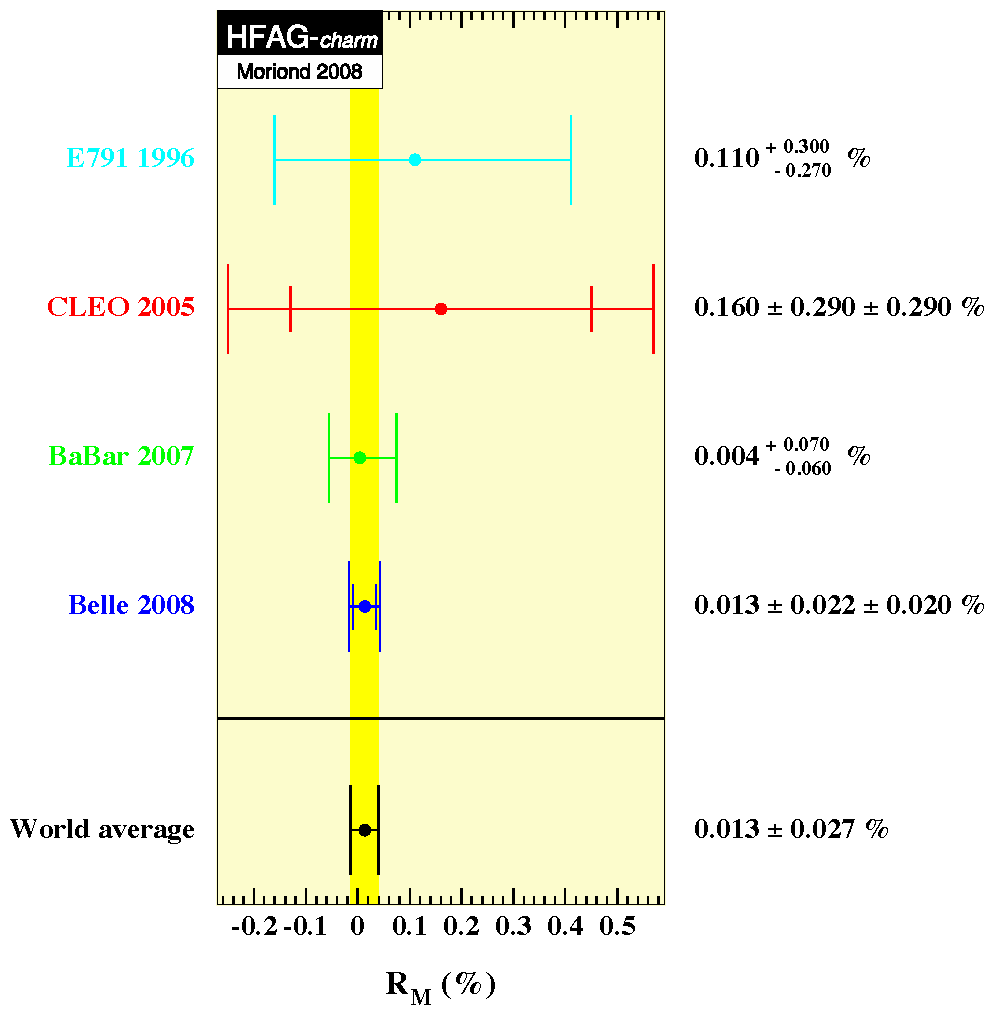
\includegraphics[width=4.2in]{figures/charm/rm_semi_9mar08}
\end{center}
\vskip-0.20in
\caption{\label{fig:rm_semi}
World average value of $R^{}_M$ from Ref.~\cite{HFAG_charm:webpage},
as calculated from $D^0\ra K^+\ell^-\nu$ 
measurements~\cite{Aitala:1996vz,Cawlfield:2005ze,Aubert:2007aa,Bitenc:2008bk}. }
\end{figure}

\begin{figure}
\begin{center}
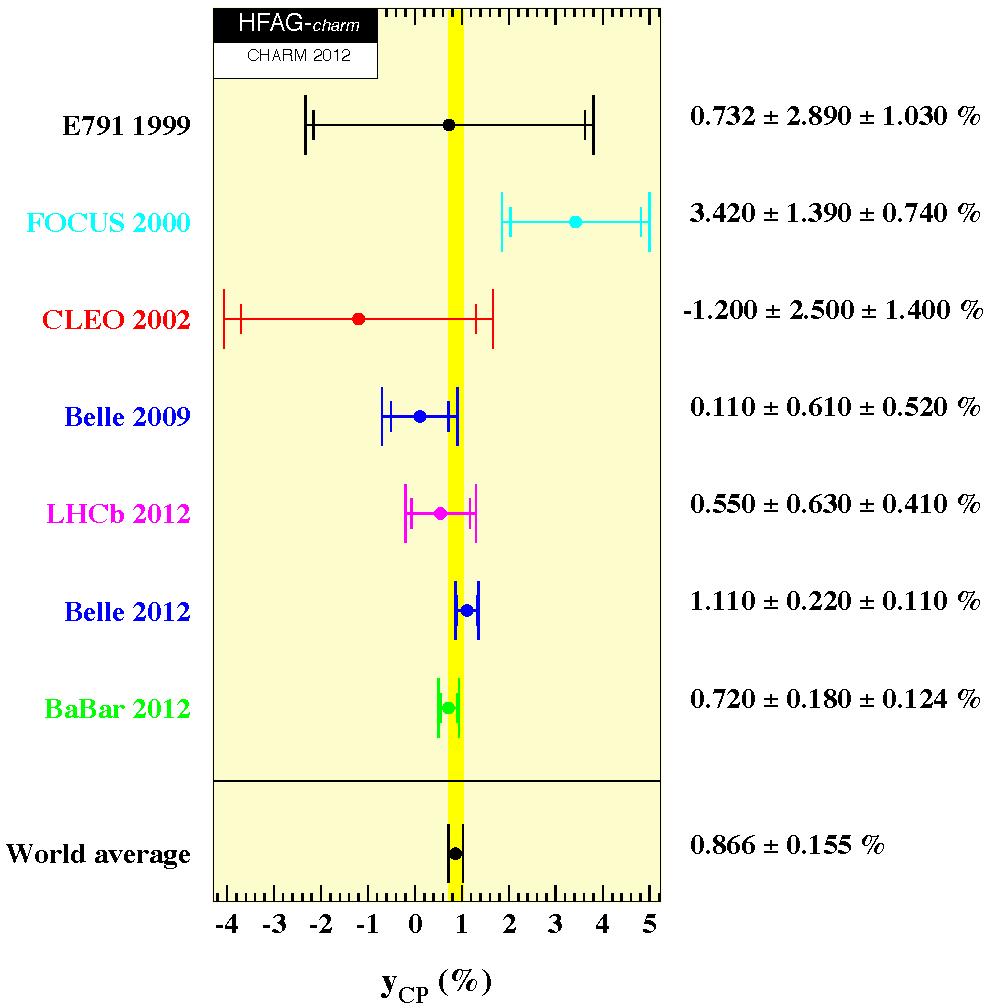
\includegraphics[width=4.2in]{figures/charm/ycp_13may12}
\end{center}
\vskip-0.20in
\caption{\label{fig:ycp}
World average value of $y^{}_{CP}$ from 
Ref.~\cite{HFAG_charm:webpage}, as calculated from \dkkpp\ 
measurements~\cite{Aitala:1999dt,Link:2000cu,Csorna:2001ww,
Zupanc:2009sy,Staric:2012ta,Lees:2012qh,Aaij:2011ad}.  }
\end{figure}


\begin{figure}
\begin{center}
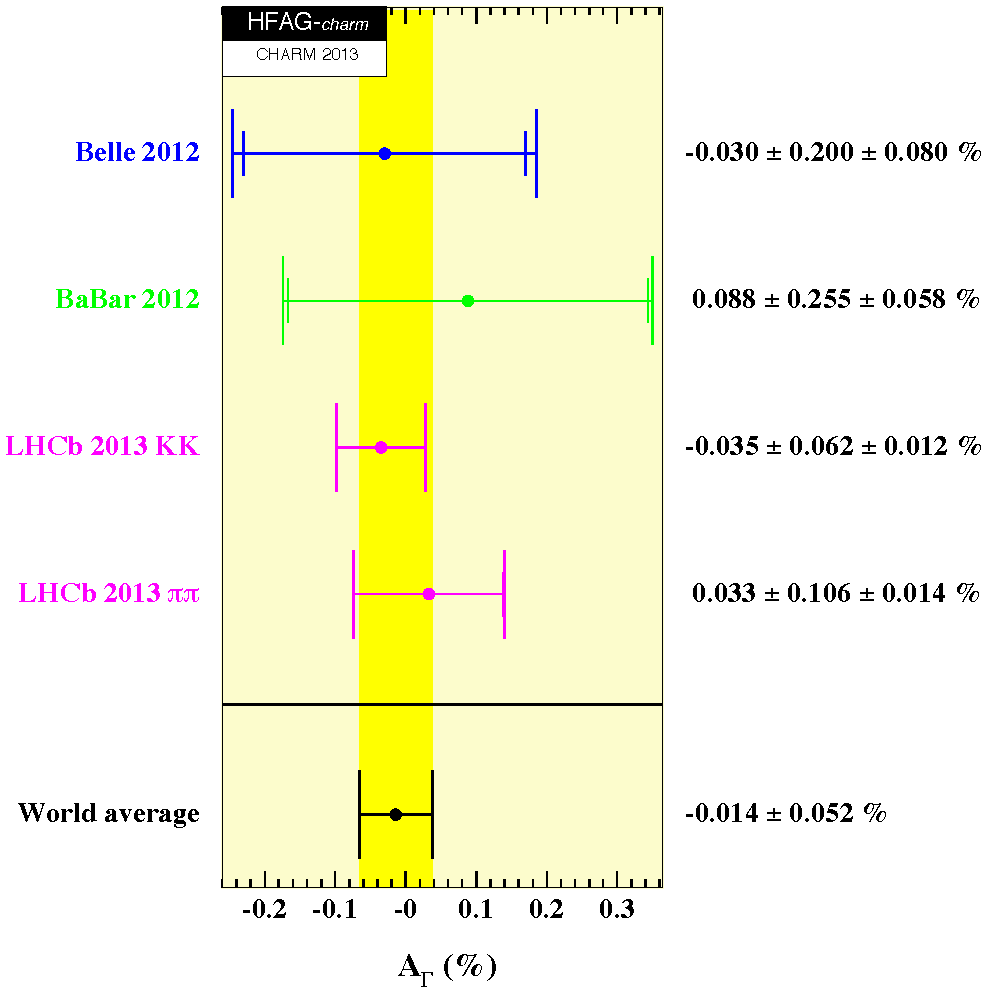
\includegraphics[width=4.2in]{figures/charm/a_gamma_31aug13}
\end{center}
\vskip-0.20in
\caption{\label{fig:Agamma}
World average value of $A^{}_\Gamma$ from 
Ref.~\cite{HFAG_charm:webpage}, as calculated from \dkkpp\ 
measurements~\cite{Staric:2012ta,Lees:2012qh,Aaij:2013ria}.}
\end{figure}


The relationships between the observables and the fitted
parameters are listed in Table~\ref{tab:relationships}. 
For each set of correlated observables we construct a
difference vector $\vec{V}$ between measured values and
those calculated from fitted parameters using the
relations of Table~\ref{tab:relationships}; \eg\ for 
$D^0\ra K^0_S\,\pi^+\pi^-$ decays,
$\vec{V}=(\Delta x,\Delta y,\Delta |q/p|,\Delta \phi)$.
%where $\Delta$ represents the difference between the 
%measured value and the fitted value.
The contribution of a set of observables to the $\chi^2$ 
is calculated as $\vec{V}\cdot (M^{-1})\cdot\vec{V}^T$, 
where $M^{-1}$ is the inverse of the covariance matrix 
for the measurement. Covariance matrices are constructed 
from the correlation coefficients among the measured observables.
These coefficients (where applicable) are also listed in 
Tables~\ref{tab:observables1}-\ref{tab:observables3}. 

\begin{table}
\renewcommand{\arraycolsep}{0.02in}
\renewcommand{\arraystretch}{1.3}
\begin{center}
\caption{\label{tab:relationships}
Left: decay modes used to determine fitted parameters 
$x,\,y,\,\delta,\,\delta^{}_{K\pi\pi},\,R^{}_D,\,A^{}_D,\,|q/p|$, and $\phi$.
Middle: the observables measured for each decay mode. Right: the 
relationships between the observables measured and the fitted
parameters. $\langle t\rangle$ is the mean lifetime for 
$D^0\ra K^+K^-$ or $D^0\ra\pi^+\pi^-$ decays.}
\vspace*{6pt}
\footnotesize
\resizebox{0.99\textwidth}{!}{
\begin{tabular}{l|c|l}
\hline
\textbf{Decay Mode} & \textbf{Observables} & \textbf{Relationship} \\
\hline
$D^0\ra K^+K^-/\pi^+\pi^-$  & 
\begin{tabular}{c}
 $y^{}_{CP}$  \\
 $A^{}_{\Gamma}$
\end{tabular} & 
$\begin{array}{c}
2y^{}_{CP} = 
\left(\left|q/p\right|+\left|p/q\right|\right)y\cos\phi - \\
\hskip0.50in \left(\left|q/p\right|-\left|p/q\right|\right)x\sin\phi \\
2A^{}_\Gamma = 
\left(\left|q/p\right|-\left|p/q\right|\right)y\cos\phi - \\
\hskip0.50in \left(\left|q/p\right|+\left|p/q\right|\right)x\sin\phi
\end{array}$   \\
\hline
$D^0\ra K^0_S\,\pi^+\pi^-$ & 
$\begin{array}{c}
x \\ 
y \\ 
|q/p| \\ 
\phi
\end{array}$ &   \\ 
\hline
$D^0\ra K^+\ell^-\nu$ & $R^{}_M$  & $R^{}_M = (x^2 + y^2)/2$ \\
\hline
\begin{tabular}{l}
$D^0\ra K^+\pi^-\pi^0$ \\
(Dalitz plot analysis)
\end{tabular} & 
$\begin{array}{c}
x'' \\ 
y''
\end{array}$ &
$\begin{array}{l}
x'' = x\cos\delta^{}_{K\pi\pi} + y\sin\delta^{}_{K\pi\pi} \\ 
y'' = y\cos\delta^{}_{K\pi\pi} - x\sin\delta^{}_{K\pi\pi}
\end{array}$ \\
\hline
\begin{tabular}{l}
``Double-tagged'' \\
branching fractions \\
measured in \\
$\psi(3770)\ra DD$ decays
\end{tabular} & 
$\begin{array}{c}
R^{}_M \\
y \\
R^{}_D \\
\sqrt{R^{}_D}\cos\delta
\end{array}$ &   $R^{}_M = (x^2 + y^2)/2$ \\
\hline
$D^0\ra K^+\pi^-$ &
$\begin{array}{c}
%R^+_D,\ R^-_D \\
x'^2,\ y' \\
x'^{2+},\ x'^{2-} \\
y'^+,\ y'^-
\end{array}$ & 
$\begin{array}{l}
%R^{}_D = (R^+_D + R^-_D)/2 \\
%A^{}_D = (R^+_D - R^-_D)/(R^+_D + R^-_D)  \\ \\
%R^\pm_M=(x'^{\pm 2}+y'^{\pm 2})/2 \\
%(|q/p|^4-1)/(|q/p|^4+1)=(R^+_M-R^-_M)/(R^+_M+R^-_M)\equiv A^{}_M \\ \\
x' = x\cos\delta + y\sin\delta \\ 
y' = y\cos\delta - x\sin\delta \\
A^{}_M\equiv (|q/p|^4-1)/(|q/p|^4+1) \\
x'^\pm = [(1\pm A^{}_M)/(1\mp A^{}_M)]^{1/4} \times \\
\hskip0.50in (x'\cos\phi\pm y'\sin\phi) \\
y'^\pm = [(1\pm A^{}_M)/(1\mp A^{}_M)]^{1/4} \times \\
\hskip0.50in (y'\cos\phi\mp x'\sin\phi) \\
%x'^\pm = |q/p|^{\pm 1}(x'\cos\phi\pm y'\sin\phi) \\
%y'^\pm = |q/p|^{\pm 1}(y'\cos\phi\mp x'\sin\phi) \\
\end{array}$ \\
\hline
\begin{tabular}{c}
$D^0\ra K^+\pi^-/K^-\pi^+$ \\
(time-integrated)
\end{tabular} & 
\begin{tabular}{c}
$\frac{\displaystyle \Gamma(D^0\ra K^+\pi^-)+\Gamma(\dbar\ra K^-\pi^+)}
{\displaystyle \Gamma(D^0\ra K^-\pi^+)+\Gamma(\dbar\ra K^+\pi^-)}$  \\ \\
$\frac{\displaystyle \Gamma(D^0\ra K^+\pi^-)-\Gamma(\dbar\ra K^-\pi^+)}
{\displaystyle \Gamma(D^0\ra K^+\pi^-)+\Gamma(\dbar\ra K^-\pi^+)}$ 
\end{tabular} & 
\begin{tabular}{c}
$R^{}_D$ \\ \\ \\
$A^{}_D$ 
\end{tabular} \\
\hline
\begin{tabular}{c}
$D^0\ra K^+K^-/\pi^+\pi^-$ \\
(time-integrated)
\end{tabular} & 
\begin{tabular}{c}
$\frac{\displaystyle \Gamma(D^0\ra K^+K^-)-\Gamma(\dbar\ra K^+K^-)}
{\displaystyle \Gamma(D^0\ra K^+K^-)+\Gamma(\dbar\ra K^+K^-)}$    \\ \\
$\frac{\displaystyle \Gamma(D^0\ra\pi^+\pi^-)-\Gamma(\dbar\ra\pi^+\pi^-)}
{\displaystyle \Gamma(D^0\ra\pi^+\pi^-)+\Gamma(\dbar\ra\pi^+\pi^-)}$ 
\end{tabular} & 
\begin{tabular}{c}
$A^{}_K  + \frac{\displaystyle \langle t\rangle}
{\displaystyle \tau^{}_D}\,{\cal A}_{CP}^{\rm indirect}$ 
\ \ (${\cal A}_{CP}^{\rm indirect}\approx -A^{}_\Gamma$)
\\ \\ \\
$A^{}_\pi + \frac{\displaystyle \langle t\rangle}
{\displaystyle \tau^{}_D}\,{\cal A}_{CP}^{\rm indirect}$ 
\ \ (${\cal A}_{CP}^{\rm indirect}\approx -A^{}_\Gamma$)
\end{tabular} \\
\hline
%2{\cal A}_{CP}^{\rm indirect} & = & 
%\Big(\left|q/p\right| + \left|p/q\right|\Big) x \sin\phi\ -\ 
%\Big(\left|q/p\right| - \left|p/q\right|\Big) y \cos\phi \\
\end{tabular}
}
\end{center}
\end{table}


\subsubsection{Fit results}

The global fit uses MINUIT with the MIGRAD minimizer, 
and all errors are obtained from MINOS~\cite{MINUIT:webpage}. 
Four separate fits are performed: 
{\it (a)}\ assuming \cp\ conservation, \ie\ fixing
$A^{}_D\!=\!0$, $A_K\!=\!0$, $A^{}_\pi\!=\!0$, $\phi\!=\!0$, 
and $|q/p|\!=\!1$;
{\it (b)}\ assuming no direct \cpv\ in doubly Cabibbo-suppressed (DCS)
decays and fitting for parameters $(x,y,|q/p|)$ or $(x,y,\phi)$; 
{\it (c)}\ assuming no direct \cpv\ in DCS decays and fitting for
alternative parameters $x^{}_{12}= 2|M^{}_{12}|/\Gamma$, 
$y^{}_{12}= \Gamma^{}_{12}/\Gamma$, and 
$\phi^{}_{12}= {\rm Arg}(M^{}_{12}/\Gamma^{}_{12})$,
where $M^{}_{12}$ and $\Gamma^{}_{12}$ are the off-diagonal
elements of the $D^0$-$\dbar$ mass and decay matrices, respectively; and
{\it (d)}\ allowing full \cpv, \ie\ floating all parameters. 

For the fits assuming no-direct-\cpv\ in DCS decays, 
we set $A^{}_D\!=\!0$. In addition, for fit 
{\it (b)\/} we impose the relation~\cite{Ciuchini:2007cw,Kagan:2009gb}
$\tan\phi = (1-|q/p|^2)/(1+|q/p|^2)\times (x/y)$, which reduces 
four independent parameters to 
three.\footnote{One can also use Eq.~(15) of Ref.~\cite{Grossman:2009mn}
to reduce four parameters to three.} 
We impose this relationship in two ways. First we float parameters
$x$, $y$, and $\phi$ and from these derive $|q/p|$; subsequently we
repeat the fit floating $x$, $y$, and $|q/p|$ and from these derive 
$\phi$. The central values returned by the two fits are identical,
but the first fit yields MINOS errors for $\phi$, while the second
fit yields MINOS errors for $|q/p|$. For no-direct-\cpv\ fit 
{\it (c)}, we fit for the underlying parameters $x^{}_{12}$, $y^{}_{12}$, 
and $\phi^{}_{12}$, from which parameters $x$, $y$, $|q/p|$, and $\phi$ 
are derived. 

All fit results are listed in 
Table~\ref{tab:results}. For the \cpv-allowed fit,
individual contributions to the $\chi^2$ are listed 
in Table~\ref{tab:results_chi2}. The total $\chi^2$ 
is 66.8 for $45-10=35$ degrees of freedom; this 
corresponds to a confidence level of~0.001,
which is uncomfortably small.

Confidence contours in the two dimensions $(x,y)$ or 
in $(|q/p|,\phi)$ are obtained by allowing, for any point in the
two-dimensional plane, all other fitted parameters to take their 
preferred values. The resulting $1\sigma$-$5\sigma$ contours 
are shown 
in Fig.~\ref{fig:contours_ncpv} for the \cp-conserving case, 
in Fig.~\ref{fig:contours_ndcpv} for the no-direct-\cpv\ case, 
and in Fig.~\ref{fig:contours_cpv} for the \cpv-allowed 
case. The contours are determined from the increase of the
$\chi^2$ above the minimum value.
One observes that the $(x,y)$ contours for the no-\cpv\ fit 
are very similar to those for the \cpv-allowed fit. In the latter
fit, the $\chi^2$ at the no-mixing point $(x,y)\!=\!(0,0)$ is 421
units above the minimum value, which, for two degrees of freedom,
corresponds to a confidence level $>11.5\sigma$.\footnote{This is
the limit of the CERNLIB PROB routine used for this calculation.}
Thus, no mixing is excluded at this high level. In the $(|q/p|,\phi)$
plot, the point $(1,0)$ is within the $1\sigma$ contour; thus the
data is consistent with \cp\ conservation.

One-dimensional confidence curves for individual parameters 
are obtained by allowing, for any value of the parameter, all other 
fitted parameters to take their preferred values. The resulting
functions $\Delta\chi^2=\chi^2-\chi^2_{\rm min}$ ($\chi^2_{\rm min}$
is the minimum value) are shown in Fig.~\ref{fig:1dlikelihood}.
The points where $\Delta\chi^2=3.84$ determine 95\% C.L. intervals 
for the parameters. These intervals are listed in Table~\ref{tab:results}.


\begin{figure}
\begin{center}
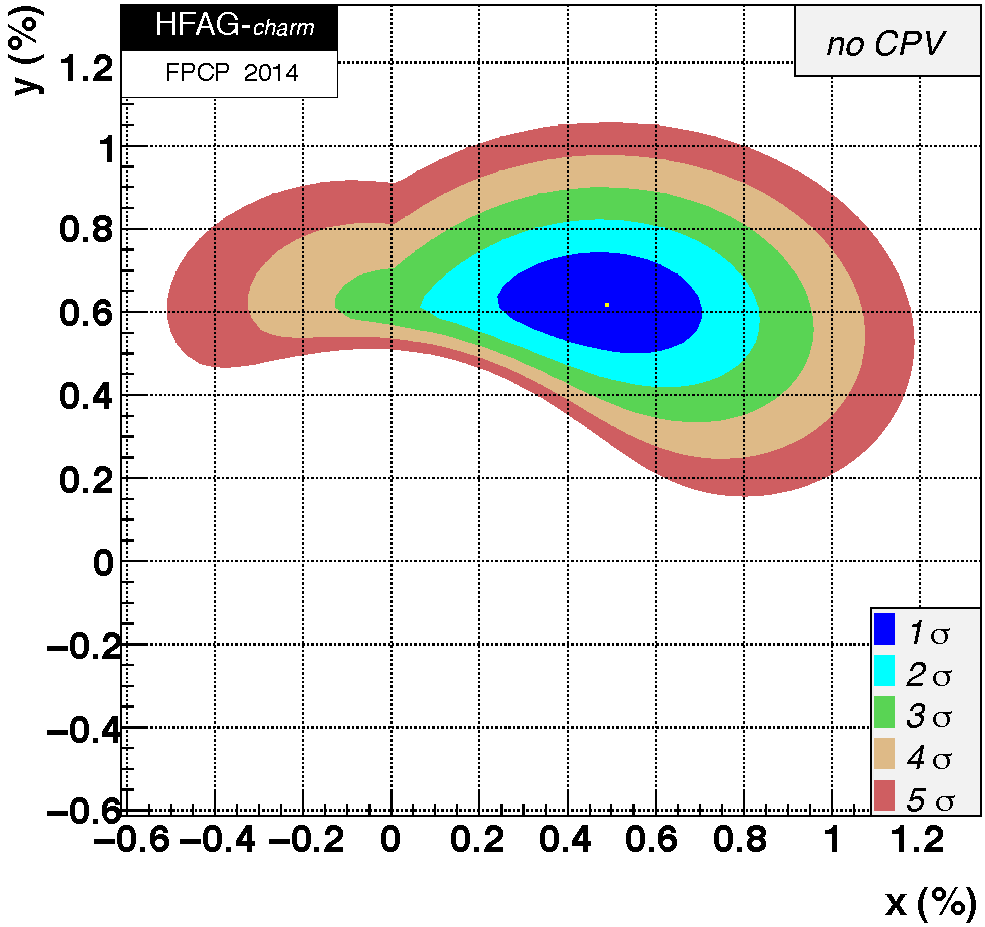
\includegraphics[width=4.2in]{figures/charm/fig_plot_xyn2d}
\end{center}
\vskip-0.20in
\caption{\label{fig:contours_ncpv}
Two-dimensional contours for mixing parameters $(x,y)$, for no \cpv. }
\end{figure}


\begin{figure}
\begin{center}
\vbox{
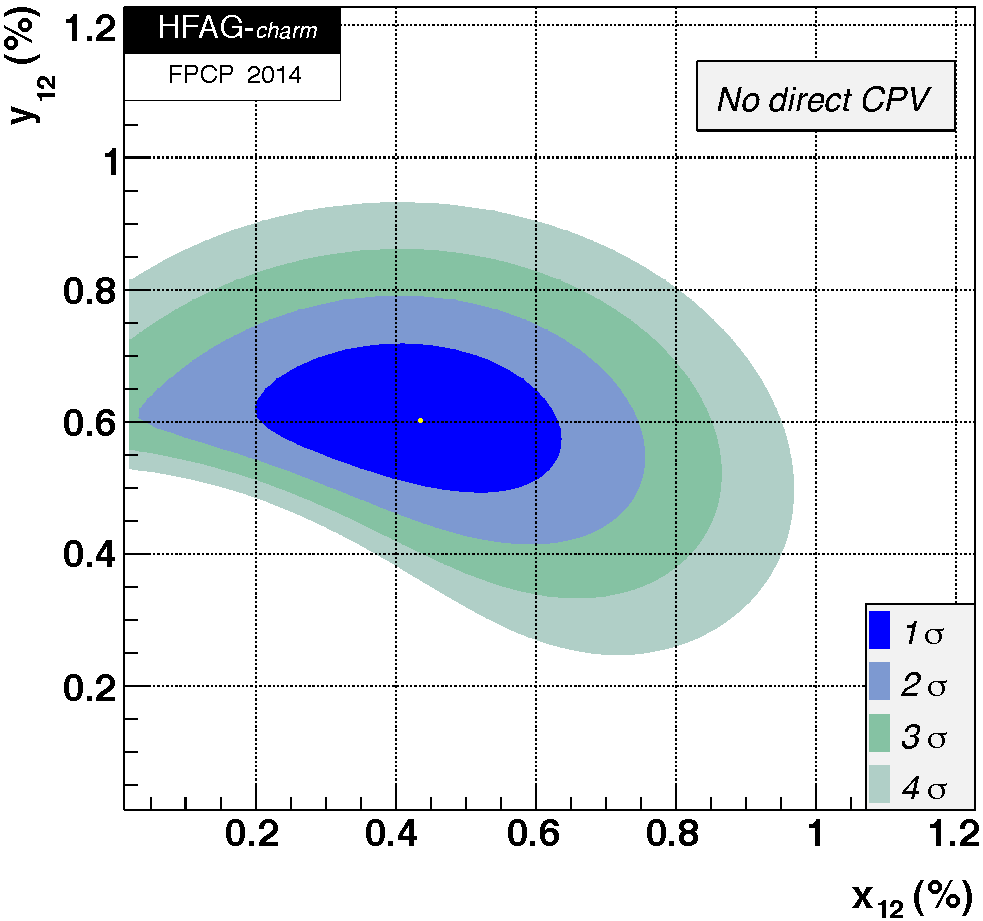
\includegraphics[width=84mm]{figures/charm/fig_plot_xy122d}
%\vskip0.10in
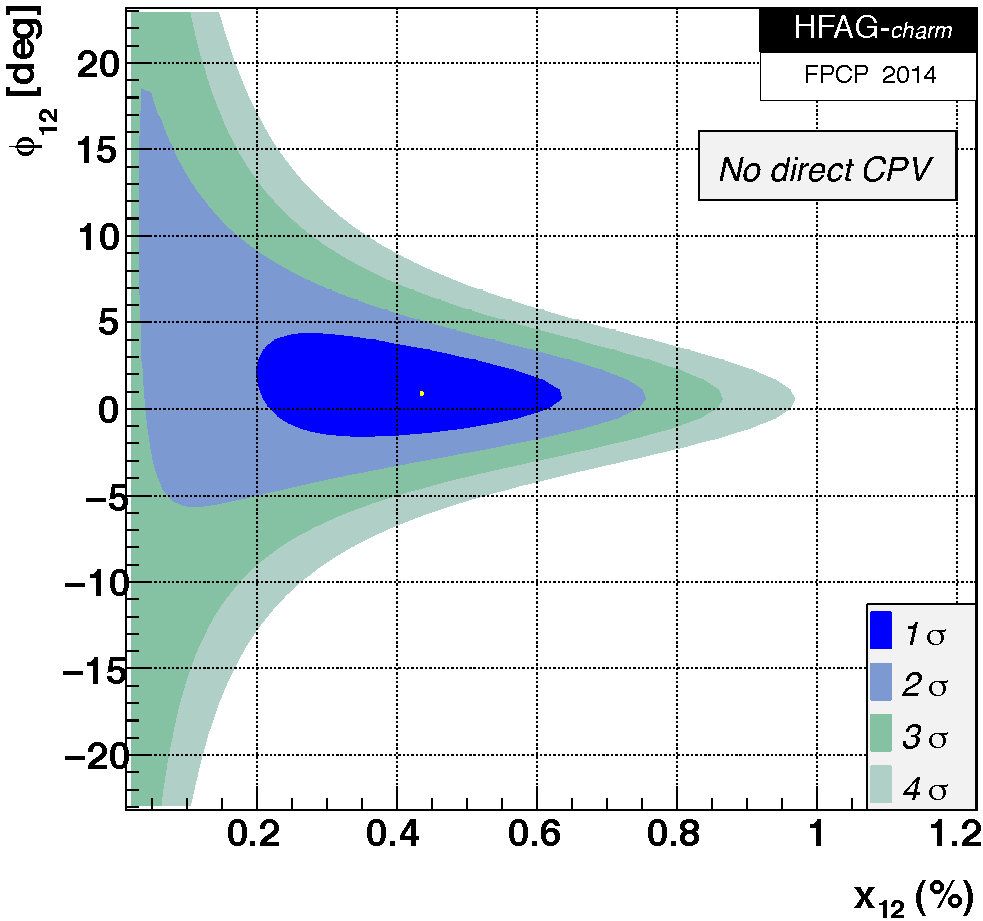
\includegraphics[width=84mm]{figures/charm/fig_plot_xp122d}
\vskip0.30in
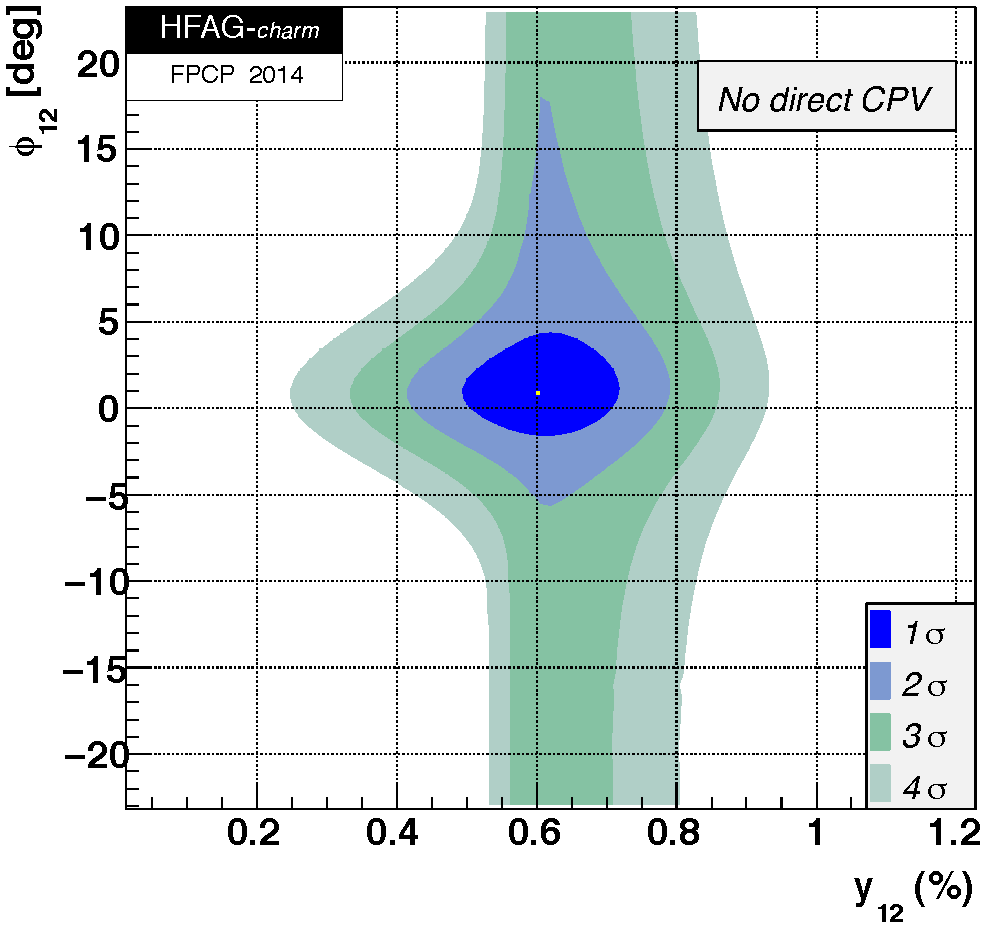
\includegraphics[width=84mm]{figures/charm/fig_plot_yp122d}
}
\end{center}
\vskip-0.10in
\caption{\label{fig:contours_ndcpv}
Two-dimensional contours for theoretical parameters 
$(x^{}_{12},y^{}_{12})$ (top left), 
$(x^{}_{12},\phi^{}_{12})$ (top right), and 
$(y^{}_{12},\phi^{}_{12})$ (bottom), 
for no direct \cpv.}
\end{figure}


\begin{figure}
\begin{center}
\vbox{
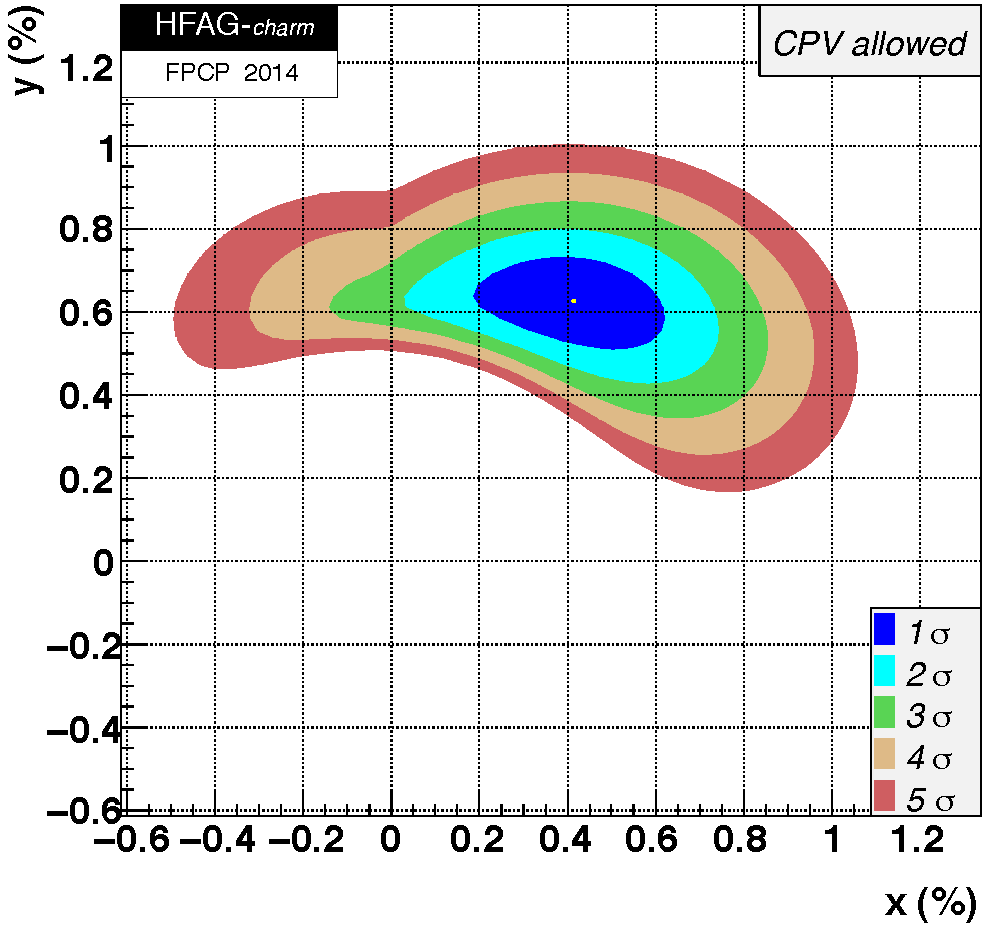
\includegraphics[width=4.2in]{figures/charm/fig_plot_xy2d}
\vskip0.10in
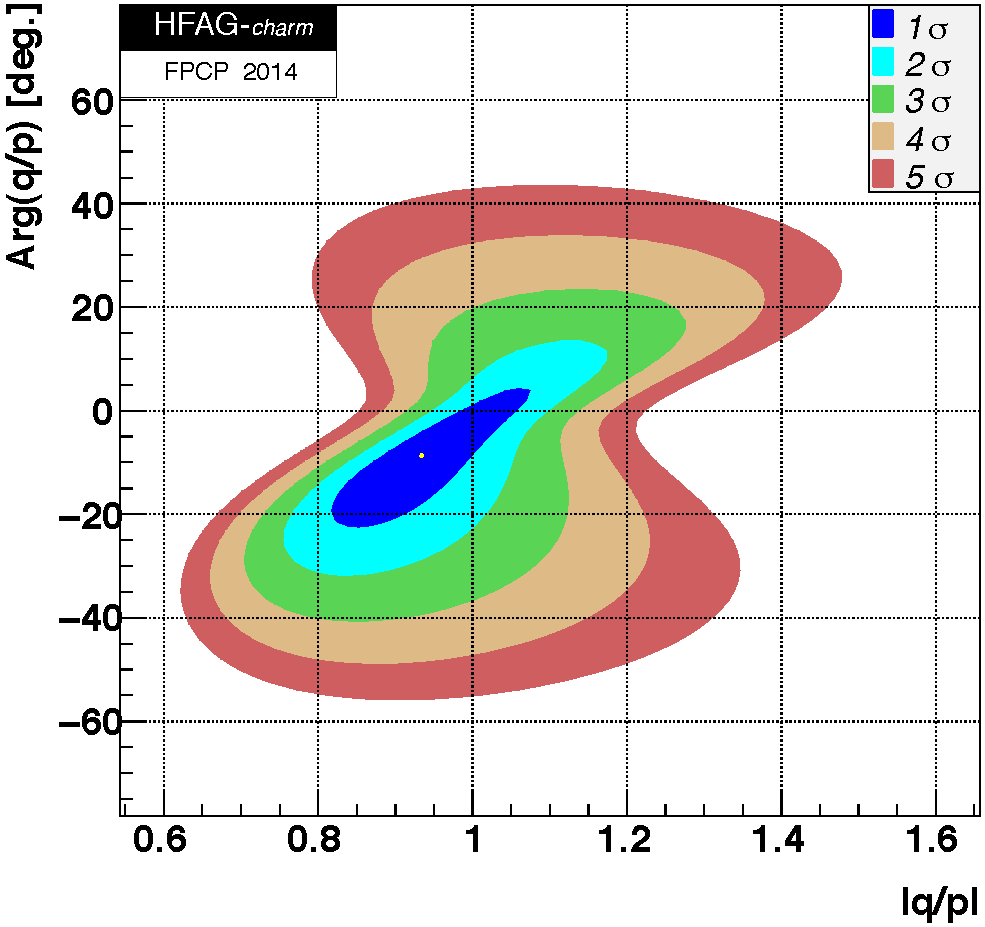
\includegraphics[width=4.2in]{figures/charm/fig_plot_qp2d}
}
\end{center}
\vskip-0.10in
\caption{\label{fig:contours_cpv}
Two-dimensional contours for parameters $(x,y)$ (top) 
and $(|q/p|,\phi)$ (bottom), allowing for \cpv.}
\end{figure}


\begin{figure}
\begin{center}
\hbox{\hskip0.50in
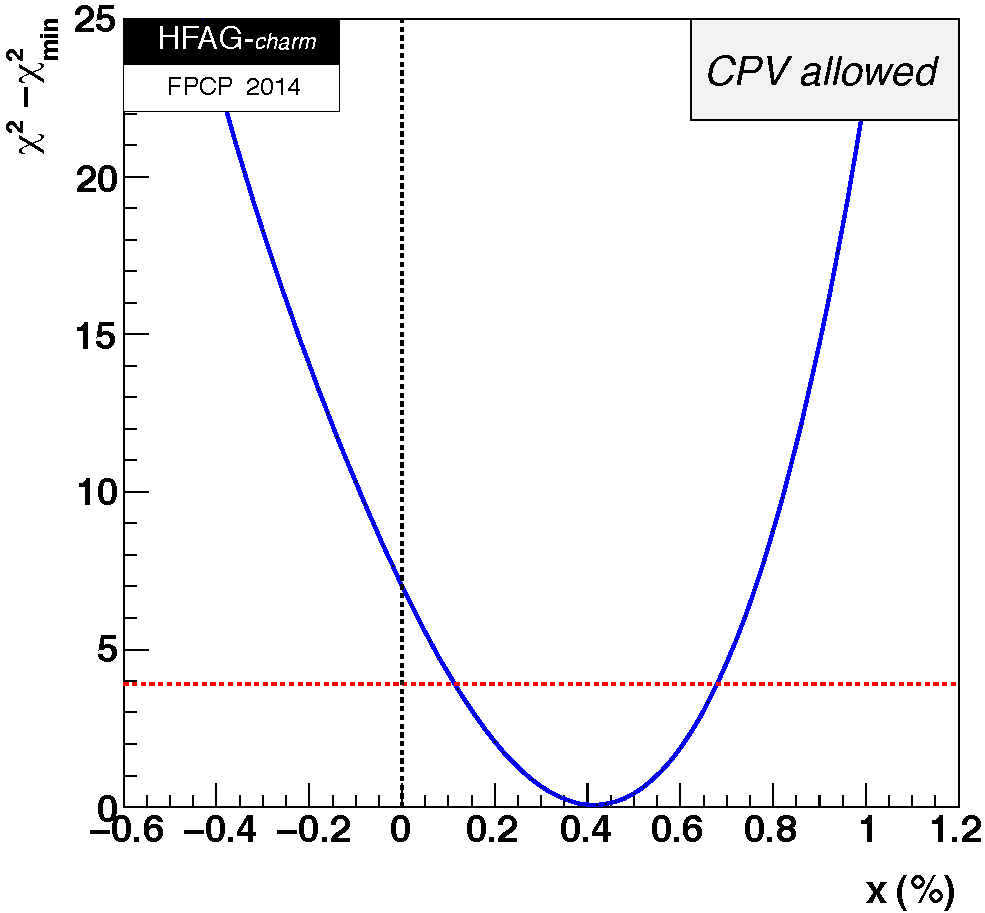
\includegraphics[width=72mm]{figures/charm/fig_plot_x1d}
\hskip0.20in
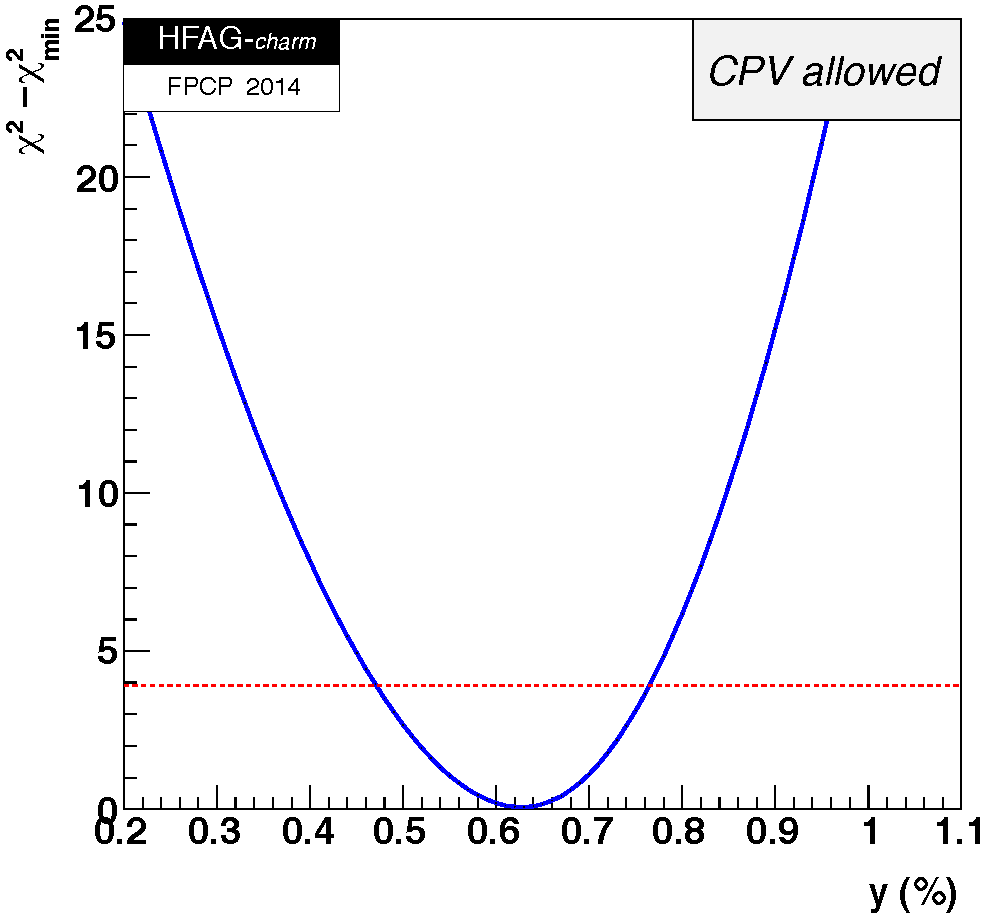
\includegraphics[width=72mm]{figures/charm/fig_plot_y1d}}
\hbox{\hskip0.50in
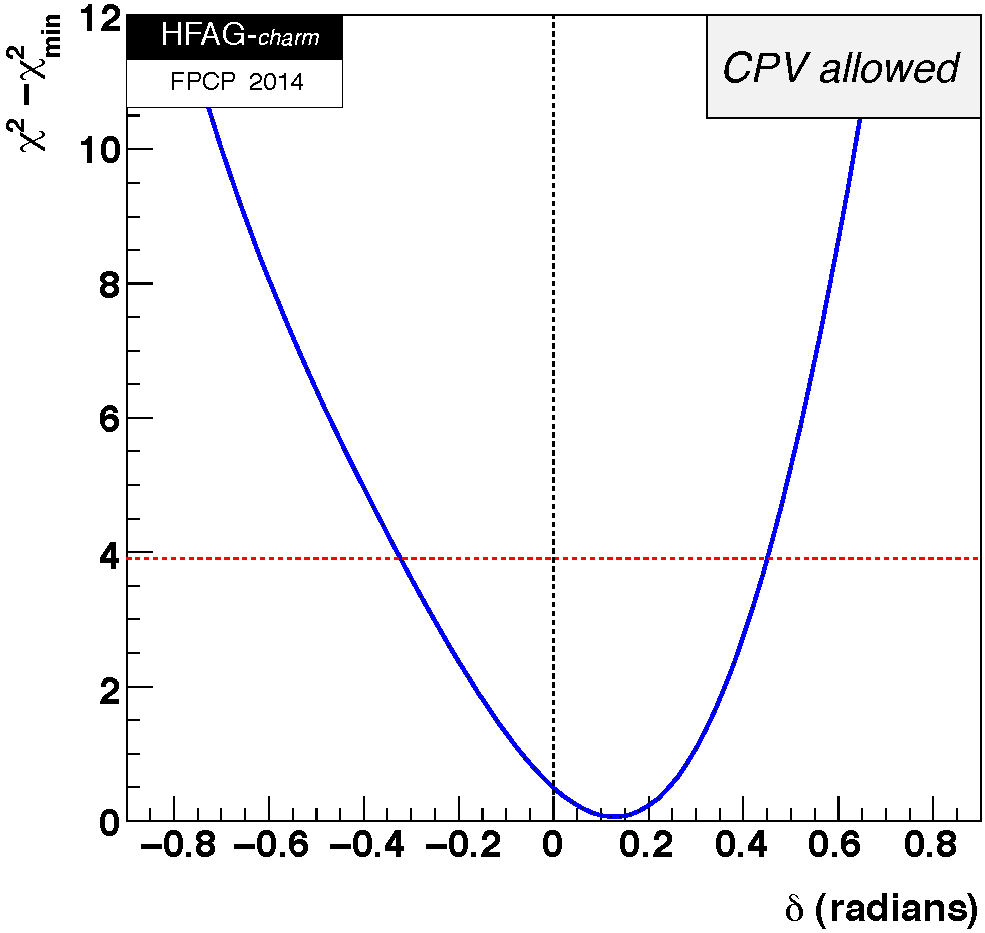
\includegraphics[width=72mm]{figures/charm/fig_plot_d1d}
\hskip0.20in
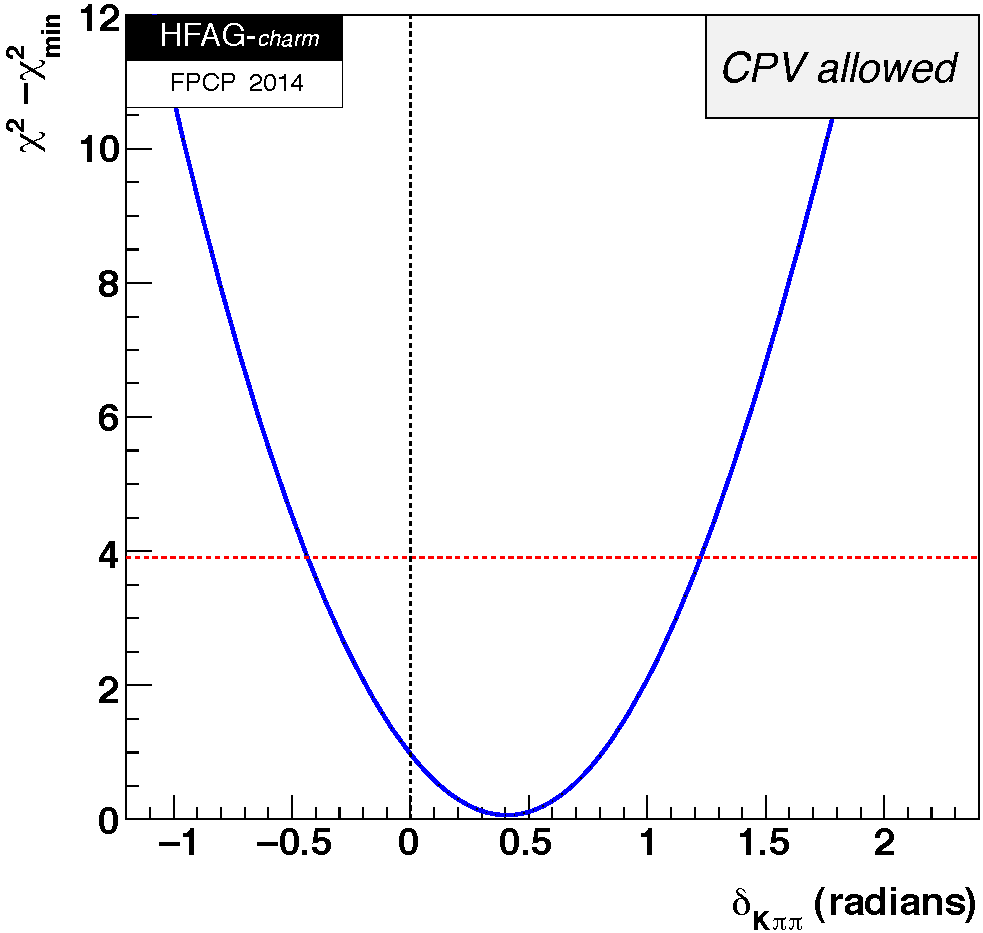
\includegraphics[width=72mm]{figures/charm/fig_plot_d21d}}
\hbox{\hskip0.50in
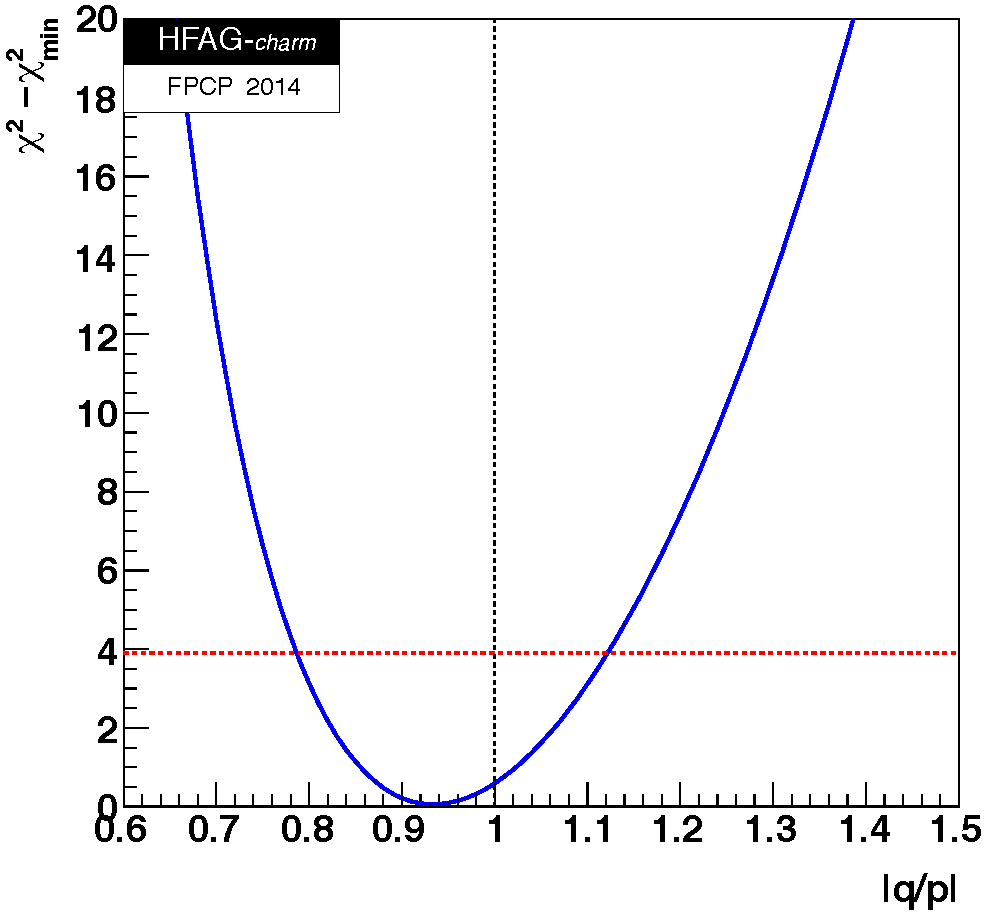
\includegraphics[width=72mm]{figures/charm/fig_plot_q1d}
\hskip0.20in
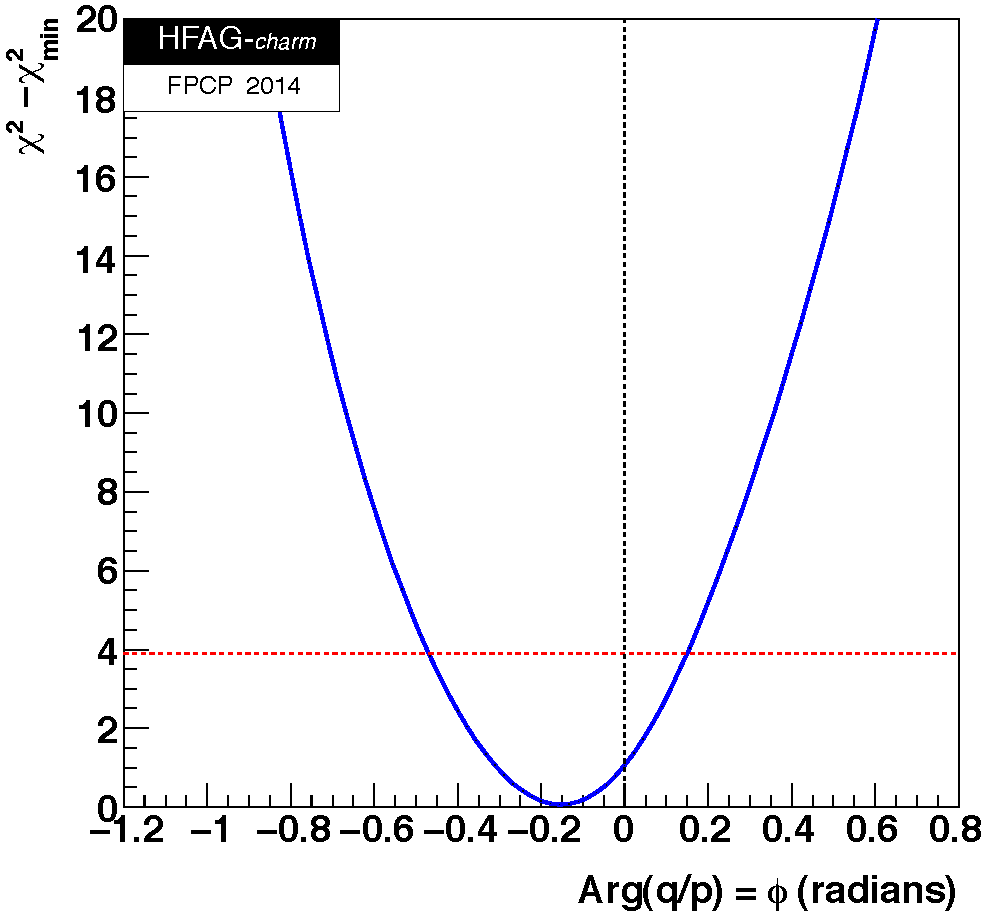
\includegraphics[width=72mm]{figures/charm/fig_plot_p1d}}
\end{center}
\vskip-0.30in
\caption{\label{fig:1dlikelihood}
The function $\Delta\chi^2=\chi^2-\chi^2_{\rm min}$ 
for fitted parameters
$x,\,y,\,\delta,\,\delta^{}_{K\pi\pi},\,|q/p|$, and $\phi$.
The points where $\Delta\chi^2=3.84$ (denoted by dashed 
horizontal lines) determine 95\% C.L. intervals. }
\end{figure}


\begin{table}
\renewcommand{\arraystretch}{1.4}
\begin{center}
\caption{\label{tab:results}
Results of the global fit for different assumptions concerning~\cpv.}
\vspace*{6pt}
\footnotesize
\begin{tabular}{c|cccc}
\hline
\textbf{Parameter} & \textbf{\boldmath No \cpv} & \textbf{\boldmath No direct \cpv} 
& \textbf{\boldmath \cpv-allowed} & \textbf{\boldmath \cpv-allowed} \\
 & & \textbf{\boldmath in DCS decays} & & \textbf{\boldmath 95\% CL Interval} \\
%\begin{tabular}{c|cc}
%\hline
%\textbf{Parameter} & \textbf{\boldmath No \cpv} & \textbf{\boldmath \cpv-allowed} \\
\hline
$\begin{array}{c}
x\ (\%) \\ 
y\ (\%) \\ 
\delta^{}_{K\pi}\ (^\circ) \\ 
R^{}_D\ (\%) \\ 
A^{}_D\ (\%) \\ 
|q/p| \\ 
\phi\ (^\circ) \\
\delta^{}_{K\pi\pi}\ (^\circ)  \\
A^{}_{\pi} (\%) \\
A^{}_K (\%) \\
x^{}_{12}\ (\%) \\ 
y^{}_{12}\ (\%) \\ 
\phi^{}_{12} (^\circ)
\end{array}$ & 
$\begin{array}{c}
0.49\,^{+0.14}_{-0.15} \\
0.62\,\pm 0.08 \\
7.8\,^{+9.6}_{-11.1} \\
0.350\,\pm 0.004 \\
- \\
- \\
- \\
18.7\,^{+23.2}_{-23.7} \\
- \\
- \\
- \\
- \\
- 
\end{array}$ &
$\begin{array}{c}
0.43\,^{+0.14}_{-0.15}\\
0.60\,\,\pm 0.07 \\
4.6\,^{+10.3}_{-12.0}\\
0.349\,\pm 0.004 \\
- \\
1.007\,^{+0.015}_{-0.014}\\
-0.30\,^{+0.58}_{-0.60} \\ 
20.8\,^{+23.9}_{-24.3} \\ 
0.11\,\pm 0.14 \\
-0.13\,\pm 0.13 \\
0.43\,^{+0.14}_{-0.15}\\
0.60\,\pm 0.07 \\
0.9\,^{+1.9}_{-1.7} 
\end{array}$ &
$\begin{array}{c}
0.41\,^{+0.14}_{-0.15}\\
0.63\,\,^{+0.07}_{-0.08}\\
7.3\,^{+9.8}_{-11.5} \\
0.349\,\pm 0.004 \\
-0.71\,^{+0.92}_{-0.95} \\
0.93\,^{+0.09}_{-0.08} \\ 
-8.7\,^{+8.7}_{-9.1} \\ 
23.3\,^{+23.9}_{-24.4} \\
0.14\,\pm 0.15 \\
-0.11\,^{+0.14}_{-0.13} \\
 \\
 \\
 \\
\end{array}$ &
$\begin{array}{c}
\left[ 0.11,\, 0.68\right] \\
\left[ 0.47,\, 0.76\right] \\
\left[ -18.5,\, 25.8\right] \\
\left[ 0.342,\, 0.356\right] \\
\left[ -2.6,\, 1.1\right] \\
\left[ 0.79,\, 1.12\right] \\\
\left[ -26.9,\, 8.6\right] \\
\left[ -24.8,\, 70.2\right] \\
\left[ -0.15,\, 0.42\right] \\
\left[ -0.37,\, 0.15\right] \\
\left[ 0.13,\, 0.69\right] \\
\left[ 0.45,\, 0.75\right] \\
\left[ -3.0,\, 6.1\right] \\
\end{array}$ \\
\hline
\end{tabular}
\end{center}
\end{table}


\begin{table}
\renewcommand{\arraystretch}{1.4}
\begin{center}
\caption{\label{tab:results_chi2}
Individual contributions to the $\chi^2$ for the \cpv-allowed fit.}
\vspace*{6pt}
\footnotesize
\begin{tabular}{l|rr}
\hline
\textbf{Observable} & \textbf{\boldmath $\chi^2$} & \textbf{\boldmath $\sum\chi^2$} \\
\hline
$y^{}_{CP}$                      & 2.57 & 2.57 \\
$A^{}_\Gamma$                    & 0.44 & 3.02 \\
\hline
$x^{}_{K^0\pi^+\pi^-}$ Belle       & 0.55 & 3.57 \\
$y^{}_{K^0\pi^+\pi^-}$ Belle       & 3.87 & 7.44 \\
$|q/p|^{}_{K^0\pi^+\pi^-}$ Belle   & 0.28 & 7.72 \\
$\phi^{}_{K^0\pi^+\pi^-}$  Belle   & 0.16 & 7.88 \\
\hline
$x^{}_{K^0 h^+ h^-}$ \babar        & 0.87 & 8.76 \\
$y^{}_{K^0 h^+ h^-}$ \babar        & 0.03 & 8.79 \\
\hline
$R^{}_M(K^+\ell^-\nu)$           & 0.14 & 8.93 \\
\hline
$x^{}_{K^+\pi^-\pi^0}$ \babar      & 7.15 & 16.08 \\
$y^{}_{K^+\pi^-\pi^0}$ \babar      & 3.99 & 20.08 \\
\hline
CLEOc                           &      &       \\
($x/y/R^{}_D/\cos\delta/\sin\delta$) 
                                & 10.08 & 30.16 \\
\hline
$R^+_D/x'{}^{2+}/y'{}^+$ \babar  & 11.66 & 41.82    \\
$R^-_D/x'{}^{2-}/y'{}^-$ \babar  &  6.02 & 47.83    \\
$R^+_D/x'{}^{2+}/y'{}^+$ Belle   &  2.13 & 49.96    \\
$R^-_D/x'{}^{2-}/y'{}^-$ Belle   &  3.18 & 53.14    \\
$R^{}_D/x'{}^{2}/y'$ CDF         &  1.15 & 54.29    \\
$R^+_D/x'{}^{2+}/y'{}^+$ LHCb    &  1.11 & 55.50    \\
$R^-_D/x'{}^{2-}/y'{}^-$ LHCb    &  1.27 & 56.67    \\
\hline
$A^{}_{KK}/A^{}_{\pi\pi}$  \babar & 0.53 & 57.19  \\
$A^{}_{KK}/A^{}_{\pi\pi}$  Belle  & 2.06 & 59.25  \\
$A^{}_{KK}/A^{}_{\pi\pi}$  CDF    & 2.64 & 61.89  \\
$A^{}_{KK}-A^{}_{\pi\pi}$  LHCb ($D^*$ tag)   
                                & 0.26 & 62.15  \\
$A^{}_{KK}-A^{}_{\pi\pi}$  LHCb ($B^0\ra D^0\mu X$ tag)
                                & 4.65 & 66.80  \\
\hline
\end{tabular}
\end{center}
\end{table}

%\newpage

\subsubsection{Conclusions}

From the fit results listed in Table~\ref{tab:results}
and shown in Figs.~\ref{fig:contours_cpv} and \ref{fig:1dlikelihood},
we conclude that:
\begin{itemize}
\item the experimental data consistently indicate that 
$D^0$ mesons undergo mixing. The no-mixing point $x=y=0$
is excluded at $>11.5\sigma$. The parameter $x$ differs
from zero by $2.4\sigma$, and $y$ differs from zero by
$9.4\sigma$. This mixing is presumably dominated 
by long-distance processes, which are difficult to calculate.
Thus, unless it turns out that $|x|\gg |y|$~\cite{Bigi:2000wn}
(which is not currently indicated), it will be difficult to
identify new physics from $(x,y)$ alone.
\item Since \ycp\ is positive, the \cp-even state is shorter-lived
as in the $K^0$-$\kbar$ system. However, since $x$ also appears
to be positive, the \cp-even state is heavier, 
unlike in the $K^0$-$\kbar$ system.
\item The LHCb and CDF experiments measured time-integrated
asymmetries that hint at {\it direct\/} \cpv\ in $D^0$ decays
(see Table~\ref{tab:observables3}). However, more statistics 
are needed to clarify this effect.
There is no evidence for \cpv\ arising from $D^0$-$\dbar$
mixing ($|q/p|\neq 1$) or from a phase difference between
the mixing amplitude and a direct decay amplitude ($\phi\neq 0$). 
\end{itemize}

